\subsection{Layer Summaries}
\label{ss:layer_summaries}

\begin{figure}[b]
\centering
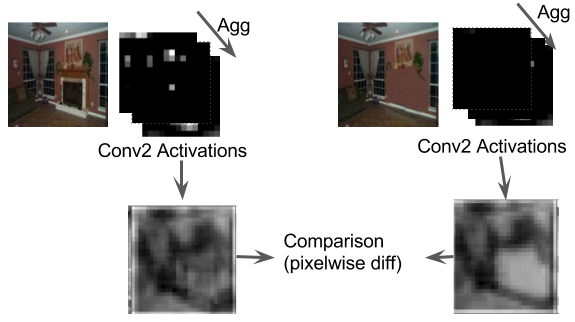
\includegraphics[width=\columnwidth]{figures/layer_summary/layer_summary_fig}
\caption{Generation of Layer Summaries for Comparison with Perturbed Images}

\label{fig:layer_summary_fig}
\end{figure}

We define a layer summary as an pixel-by-pixel aggregation over the activations images in a layer of a CNN. For instance, the \texttt{conv4} layer of Alexnet~\cite{alexnet} contains 256 distinct $14 \times 14$ activation images. We generate a layer summary by aggregating over each pixel across the set of activation images in a given layer. Layer summaries are useful for comparing the activations of an image and a perturbed version of the image as in Figure ~\ref{fig:layer_summary_fig}. We hypothesize that in a good model, that is, where a perturbation in the image does not cause a change in the output class, the difference between summaries of an original image and a perturbed image should be less apparent in later layers of the network. In a poorly performing network, however, a perturbation will propagate to the deeper layers, and ultimately change the classification decision. 

Different aggregation functions reveal different properties of a set of activation images. For instance, an average has a contribution from all activations, but makes it difficult to detect large changes in a single activation image. Conversely, a maximum over the images is sensitive to the changes in a single activation and is unable to detect changes that occur over large sets of activations. We explore the trade-offs of the choice of aggregation in the Section ~\ref{sec:exp_layer_summaries}.
